\documentclass{article}
\usepackage{tikz}
\usepackage{xcolor}

\definecolor{myblue}{RGB}{45,115,165}
\definecolor{bggray}{RGB}{240,240,240}
\definecolor{gridgray}{RGB}{180,180,180}

\begin{document}

\begin{center}
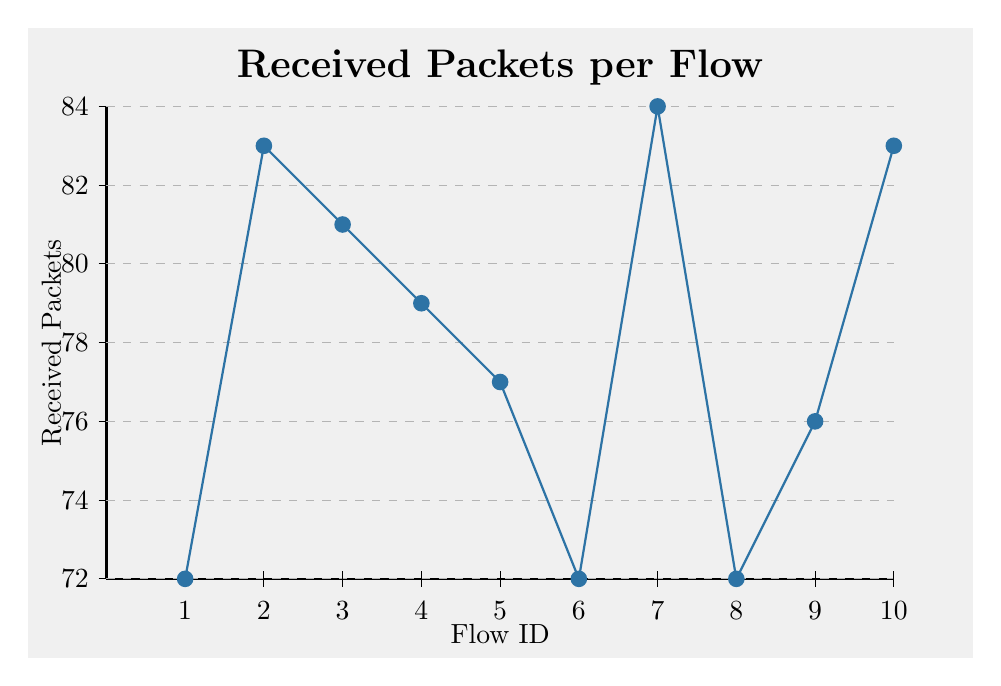
\begin{tikzpicture}

% Background
\fill[bggray] (0,0) rectangle (12,8);

% Axes
\draw[thick] (1,1) -- (1,7); % Y-axis
\draw[thick] (1,1) -- (11,1); % X-axis

% Title
\node[font=\Large\bfseries] at (6,7.5) {Received Packets per Flow};

% Labels
\node at (6,0.3) {Flow ID};
\node[rotate=90] at (0.3,4) {Received Packets};

% Y-axis ticks + grid
\foreach \y/\val in {
1/72,2/74,3/76,4/78,5/80,6/82,7/84
} {
    \draw (0.9,\y) -- (1.1,\y);
    \node[left] at (0.9,\y) {\val};
    \draw[dashed, gridgray] (1,\y) -- (11,\y);
}

% X-axis ticks (1–10)
\foreach \x in {2,3,4,5,6,7,8,9,10,11} {
    \draw (\x,0.9) -- (\x,1.1);
}
\foreach \x/\val in {
2/1,3/2,4/3,5/4,6/5,7/6,8/7,9/8,10/9,11/10
} {
    \node at (\x,0.6) {\val};
}

% Scaling (72–84 mapped to 1–7)
\def\scale{0.5}

% Data points
\coordinate (p1) at (2,{1 + (72-72)*\scale});
\coordinate (p2) at (3,{1 + (83-72)*\scale});
\coordinate (p3) at (4,{1 + (81-72)*\scale});
\coordinate (p4) at (5,{1 + (79-72)*\scale});
\coordinate (p5) at (6,{1 + (77-72)*\scale});
\coordinate (p6) at (7,{1 + (72-72)*\scale});
\coordinate (p7) at (8,{1 + (84-72)*\scale});
\coordinate (p8) at (9,{1 + (72-72)*\scale});
\coordinate (p9) at (10,{1 + (76-72)*\scale});
\coordinate (p10) at (11,{1 + (83-72)*\scale});

% Line
\draw[myblue, thick]
(p1)--(p2)--(p3)--(p4)--(p5)--(p6)--(p7)--(p8)--(p9)--(p10);

% Circular markers
\foreach \p in {p1,p2,p3,p4,p5,p6,p7,p8,p9,p10} {
    \fill[myblue] (\p) circle (3pt);
}

\end{tikzpicture}
\end{center}

\end{document}